What is the relationship between a Transnational Entrepreneur's network and their knowledge diffusion within the context of the Berlin Startup sphere.

%%%%%%%%%%%%%%%%%%%%%%%%%%%%%%%%%%%%%%%%%%%%%%%%%%%%%%%%%%%%%%%%%%%%%%%%%%%%%%%%
\section{The Theoretical Model}
%%%%%%%%%%%%%%%%%%%%%%%%%%%%%%%%%%%%%%%%%%%%%%%%%%%%%%%%%%%%%%%%%%%%%%%%%%%%%%%%
The theoretical model indicates that knowledge diffusion within a Transnational Entrepreneur's network is moderated by their network distribution. Below we will summarize the premises necessary to come to this conclusion and how we will systematically build our logic to this testable hypothesis.
\begin{figure}[!ht]
  \centering
  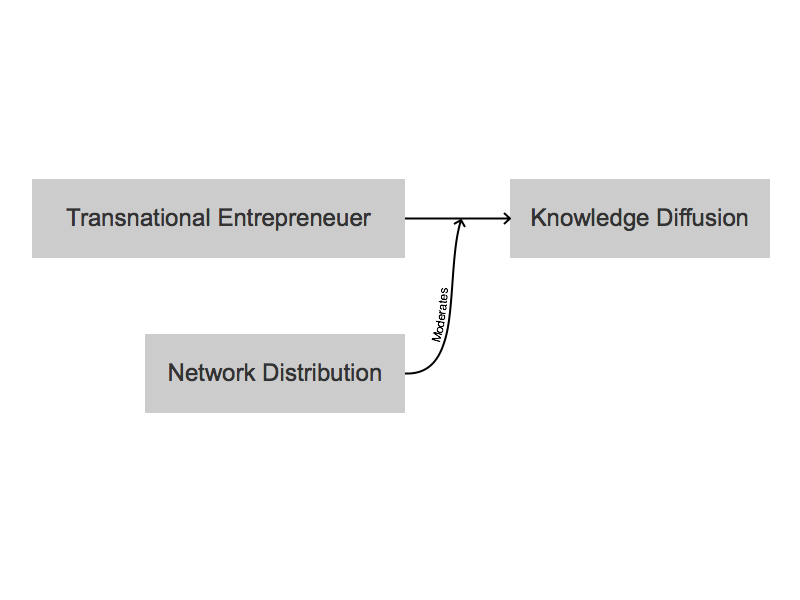
\includegraphics[width=1.0\textwidth]{theoretical_model.png}
  \caption{Knowledge Diffusion is moderated by Network Distribution.}
\end{figure}

%%%%%%%%%%%%%%%%%%%%%%%%%%%%%%%%%%%%%%%%%%%%%%%%%%%%%%%%%%%%%%%%%%%%%%%%%%%%%%%%
\section{Premises}
%%%%%%%%%%%%%%%%%%%%%%%%%%%%%%%%%%%%%%%%%%%%%%%%%%%%%%%%%%%%%%%%%%%%%%%%%%%%%%%%
The following premises are things we must accept to answer the research question. They are the set of Hypothesis upon which our research is based.
\subsection{Premise: Transnational Entrepreneur}
There exist a set of individuals that fit the criteria of a Transnational Entrepreneur. The criteria are that the entrepreneur leverages two or more networks in their business. 
\subsection{Premise: Transnational Diffusion}
The hypothesis postulates that Transnational Entrepreneurs diffuse knowledge across national borders.
\subsection{Premise: Transnational Diffusion Moderated by Network}
The frequency of knowledge diffusion across borders within a Transnational Entrepreneur's network is moderated by their network's nationality distribution. The national distribution refers to the relative populations of different populations as constrained by nationality.
\subsection{Premise: Network Distribution Normalization \& Transnational Diffusion are Positively Correlated}
The closer the Transnationl Entrepreneur's network demographics are to a normalized distribution, the higher the frequency of transnational diffusion. A normalized distribution is defined within a statistical context. This means that 32\% of a user's network should fall within one distribution, another 32\% within another. Following this same reasoning, 95\% of a given Transnational Entrepreneur's network should fall within four discrete countries.
\begin{figure}[!ht]
  \centering
  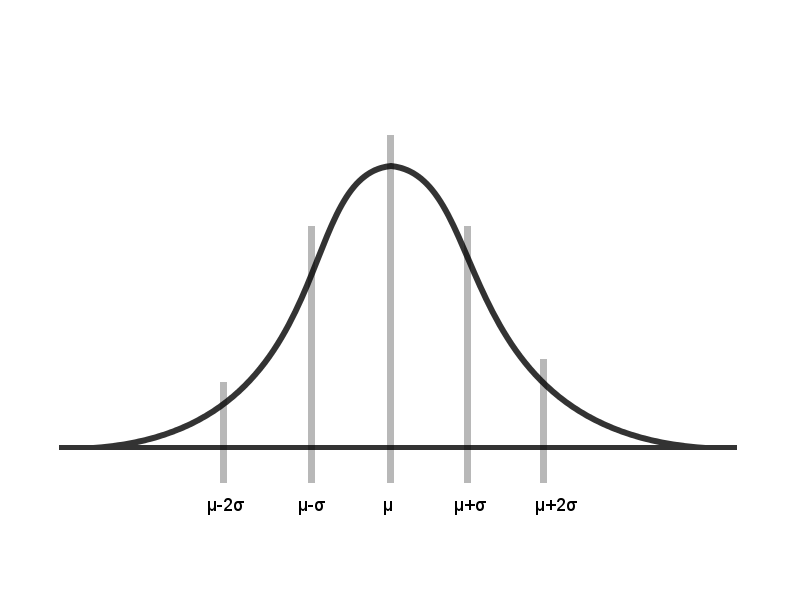
\includegraphics[width=1.0\textwidth]{normal_distribution.png}
  \caption{Normalized distribution (not drawn to scale).}
\end{figure}
